\documentclass[11pt,a4paper]{article}
\usepackage[a4paper,margin=22mm]{geometry}
\usepackage[T1]{fontenc}
\usepackage[utf8]{inputenc}
\usepackage[british]{babel}
\usepackage{newtxtext,newtxmath}
\usepackage{microtype,setspace}
\setstretch{1.12}
\usepackage{amsmath,bm}
\usepackage{booktabs,longtable,tabularx,array,ragged2e}
\usepackage{graphicx}
\graphicspath{{figures/}}
\usepackage{caption,float,enumitem,xcolor}
\captionsetup{font=small,labelfont=bf,labelsep=period,justification=justified,singlelinecheck=false}
\usepackage[numbers,sort&compress]{natbib}
\usepackage[colorlinks=true,linkcolor=black,citecolor=black,urlcolor=black]{hyperref}
\setlength{\parindent}{1.2em}
\setlength{\parskip}{0pt}
\setlength{\emergencystretch}{2em}
\setlength{\tabcolsep}{3pt}
\renewcommand{\arraystretch}{1.12}
\newcolumntype{L}[1]{>{\RaggedRight\arraybackslash}p{#1}}
\newcommand{\vect}[1]{\bm{#1}}
\renewcommand{\thefigure}{S\arabic{figure}}
\renewcommand{\thetable}{S\arabic{table}}
\addto\captionsbritish{\renewcommand{\refname}{Supplementary references}}

\title{\textbf{Supplementary material}\\[0.3em]
\large From routine cine CMR to regional myocardial dysfunction}
\author{Ziying Huo}
\date{8 October 2026}

\begin{document}
\maketitle
\vspace{1.2em}

\section*{Supplementary Methods: search boundary and evidence handling}

The review is a targeted critical narrative synthesis. It must not be described as systematic or PRISMA compliant. The inherited historical record used PubMed, Europe PMC and OpenAlex with a 1 September 2026 cutoff. Eighteen query--database combinations were run; the logs report 41 PubMed, 244 Europe PMC and 508 OpenAlex hits before export limits and deduplication. The exported working set contained 281 rows and 253 unique candidates. Twenty-one records were retained and 232 were excluded at title/available-abstract/metadata stage. A targeted top-up on 9 September, using the same historical cutoff, added two near-neighbour records, yielding 23 records representing 22 studies. This was a single AI-assisted screening stream: there was no independent duplicate human screening, no claim that all candidates were read in full and no final-stage full-text exclusion count.

The separate supplied research archive contained 40 exploratory web queries and two Europe PMC metadata queries and yielded 42 auxiliary leads. The 42 leads are counted as leads only: they are neither fully read articles nor independent cohorts nor clinical validation studies, and they are not added to the historical search denominator. They included method papers, simulations, datasets, abstracts and resources that could share participants. A further targeted source-verification update ran through 8 October 2026; it checked defined claims and validation-resource metadata, without repeating systematic screening. The exact inherited records are included in the source package at \texttt{supplementary/historical/search-record.md}, \texttt{gap-search-query-log.csv} and \texttt{near-neighbour-matrix.csv}; v9 queries and dated return records are reported separately in the QA search log.

For the present revision, central claims were rechecked against primary full text where accessible. Exact-title and DOI searches were used for StrainNet, the multivendor tagging comparison, the DENSE/tagging/feature-tracking comparison, the cine--DENSE comparison, Strain-8, reconstruction examples (CineVN, REGAIN, DENT and model-based DLR versus compressed sensing), recent finite-element and physics-informed methods, Fourier-Net+, CardioMorphNet and the 2026 single-slice DENSE/cine study. Official sources were used for CMRxRecon2025 release and modality statements. Adjacent reviews published from 2024 to 2026 were checked to position the contribution without claiming priority.

Reading depth is recorded in the separate evidence ledger. ``Full text'' means that the relevant methods, results, tables, discussion and limitations were inspected; it does not imply line-by-line duplicate review. ``Abstract/metadata'' supports only publication status, study design and results stated in that abstract. ``Not inspected'', ``not reported'' and ``not validated'' are kept distinct. Entries in Supplementary Table~\ref{tab:s3-methods} are abstract- or metadata-level readings of the cited method papers unless the main text states a deeper reading; they describe each study's own reported evaluation and are not a re-analysis.

\section*{Supplementary Note 1: strain definitions and comparison traps}

Let \(\boldsymbol\varphi:\Omega_0\rightarrow\Omega_t\) map a reference position \(\vect X\) to its deformed position \(\vect x\). The displacement is
\begin{equation}
\vect u(\vect X,t)=\boldsymbol\varphi(\vect X,t)-\vect X,
\end{equation}
and the deformation gradient is
\begin{equation}
\vect F=\frac{\partial\boldsymbol\varphi}{\partial\vect X}=\vect I+\frac{\partial\vect u}{\partial\vect X}.
\end{equation}
Common finite-strain measures include the right Cauchy--Green tensor \(\vect C=\vect F^{\mathsf T}\vect F\), Green--Lagrange strain \(\vect E=(\vect C-\vect I)/2\), and logarithmic strain obtained from a stretch tensor. In one dimension, engineering strain \(e=(\ell-\ell_0)/\ell_0\) and Green--Lagrange strain satisfy \(E=e+e^2/2\). Numerically comparing values without converting the definitions can create an apparent method bias\cite{wehner2018}.

Cardiac components require a coordinate frame. Circumferential, radial and longitudinal axes can be defined at the reference state, updated through time or constructed from a ventricular centreline. Local axes become unstable near the apex and can vary with segmentation. A transmural average differs from endocardial strain because deformation varies through the wall. Two-dimensional short-axis analyses omit longitudinal and through-plane derivatives; a reported radial or circumferential component is consequently conditional on the 2D model.

Peak definitions also differ. If \(E_s(t)\) is the segment-average strain curve, \(\min_t E_s(t)\) is generally not equal to the spatial average of pointwise minima. ``End-systolic'', ``peak systolic'' and ``peak over the whole cardiac cycle'' may diverge in dyssynchrony or post-systolic shortening. A reproducible comparison must fix the order of differentiation, projection, spatial averaging and temporal peak selection. Supplementary Figure~\ref{fig:supp-definitions} illustrates these four traps.

\begin{figure}[H]
\centering
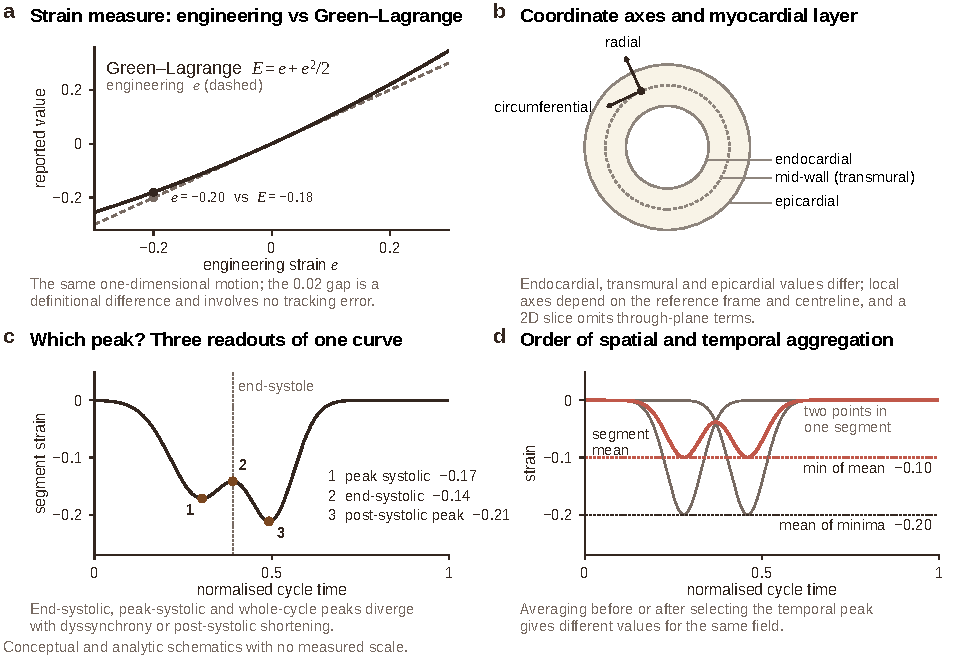
\includegraphics[width=\textwidth]{Figure_S1_strain_definition_traps.pdf}
\caption{The same motion gives different numbers under different definitions. (a) Engineering strain \(e\) and Green--Lagrange strain \(E=e+e^2/2\) differ by 0.02 at \(e=-0.20\). (b) Endocardial, mid-wall and epicardial layers and local radial and circumferential axes. (c) One segmental curve read as peak systolic, end-systolic and post-systolic peak. (d) The minimum of a segment-mean curve differs from the mean of pointwise minima. Conceptual and analytic schematics with no measured scale. Drawn programmatically (Python/matplotlib and Typst/CeTZ) with AI assistance (Claude Code, Anthropic); no generative image model was used. Author verification is required before submission.}
\label{fig:supp-definitions}
\end{figure}

\section*{Supplementary Note 2: validation targets}

The claim boundaries for common validation targets are summarised in Figure~5a of the main text.

A validation hierarchy should not be interpreted as a single ranking. Simulation supplies exact truth but imperfect realism. DENSE and tagging provide material-sensitive in-vivo information but have sequence- and processing-specific error. Scan--rescan establishes precision. LGE and outcomes test biological or clinical relationships. A mature claim often needs several targets because their weaknesses are complementary.

When two acquisitions are compared, acquisition registration is part of the reference. Slice position, breath-hold, loading and heart-rate differences can create apparent algorithm error. Where reference processing includes smoothing or temporal fitting, its effective resolution should be reported. Segment-level analyses require participant-aware uncertainty estimates because segments from one heart are correlated.

\section*{Supplementary Note 3: error attributes and mapping validity}

The distinct spatial, temporal and field-validity failure modes are illustrated in Supplementary Figure~\ref{fig:supp-errors}.

\begin{figure}[H]
\centering
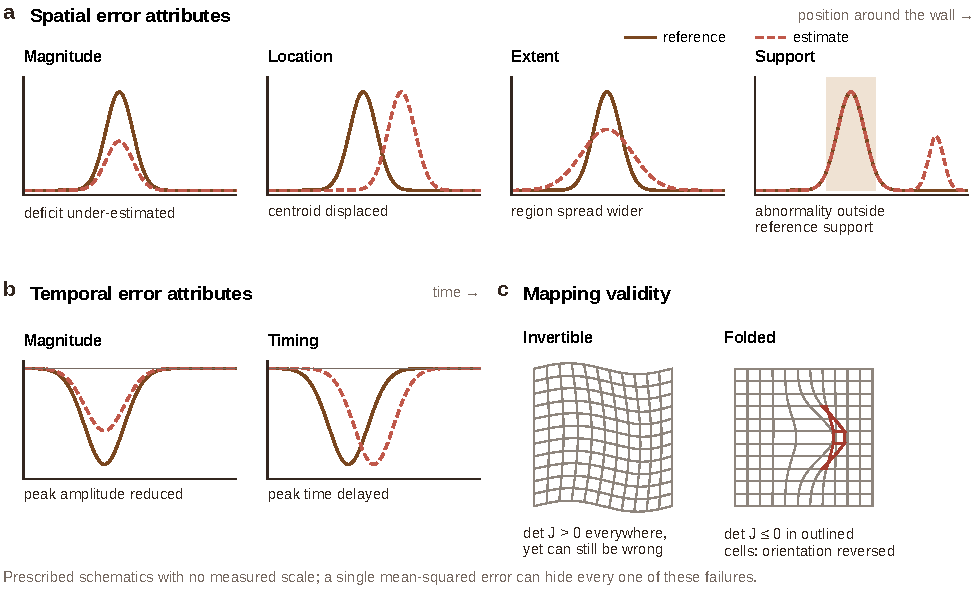
\includegraphics[width=\textwidth]{Figure_S2_error_attributes_mapping_validity.pdf}
\caption{Regional error attributes and mapping validity. (a) Reference and estimate profiles separating magnitude, location, extent and support errors. (b) Temporal magnitude and timing errors. (c) A smooth invertible mapping (\(\det J>0\)), which can still be wrong, and a folded mapping with \(\det J\le 0\) in the outlined cells. Prescribed schematics with no measured scale. Drawn programmatically (Python/matplotlib and Typst/CeTZ) with AI assistance (Claude Code, Anthropic); no generative image model was used. Author verification is required before submission.}
\label{fig:supp-errors}
\end{figure}

Let a prescribed abnormality field be \(g_{\mathrm{ref}}(\vect x,t)\) and an estimate be \(g_{\mathrm{est}}(\vect x,t)\). A single mean-squared error can conceal clinically different failures. Attribute-specific losses may include:
\begin{itemize}
\item magnitude error in an agreed region;
\item distance between abnormality centroids or peaks;
\item width, area or overlap error of a thresholded abnormal region;
\item onset, peak-time or curve-alignment error; and
\item error conditional on the reference support and a sensitivity analysis over the threshold.
\end{itemize}

Field validity is related but distinct. A positive Jacobian determinant is a useful check against local folding, while near-incompressibility may be physiologically motivated. Neither proves accurate correspondence. A smooth, invertible mapping can be wrong, and a reference generated by an approximate 2D model can violate three-dimensional tissue behaviour. Validity metrics should accompany, not replace, regional accuracy metrics.

\section*{Supplementary Note 4: learning target and control point}

DeepStrain and StrainNet illustrate why the target matters. DeepStrain demonstrated a complete automated workflow with segmentation, motion estimation, volumetric agreement, reference ranges and repeatability analyses\cite{morales2021}. Its cine motion network was not independently validated against dense material displacement for every regional claim. StrainNet used DENSE phase-derived displacement as a supervised target, but it reported two distinct evaluations\cite{wang2023strainnet}. In the 62-person independent test set, its \(0.75\pm0.35\)-mm pixelwise EPE was obtained when DENSE-magnitude contours, not cine contours, were supplied to the network and compared with DENSE displacement over myocardium and time. Separately, bSSFP cine feature-tracking contours were used for the end-systolic global and AHA-segmental circumferential-strain comparison in 59 test participants. Thus the EPE and cine-contour ICCs must not be fused into one ``cine displacement'' result; population, contour source, registration, direction, aggregation and time-point still bound the claim.

Training-time and inference-time controls must also be distinguished. Changing a loss weight usually requires matched retraining, and varying it only at test time has no effect unless the trained model exposes that parameter. Post-processing strength or a biomechanical solve, by contrast, can be a genuine inference-time control. Evaluation should compare like with like, hold splits and estimands fixed, and keep final test cases out of model or rule selection.

Supplementary Figure~\ref{fig:supp-controls} shows the two control points and their shared held-out evaluation contract.

\begin{figure}[H]
\centering
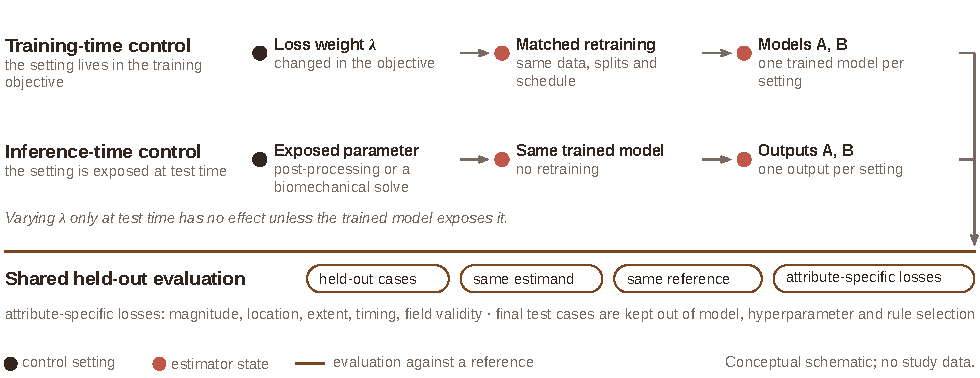
\includegraphics[width=\textwidth]{Figure_S3_training_vs_inference_controls.pdf}
\caption{Training-time versus inference-time controls. A training-loss weight requires matched retraining; a test-time parameter can be varied only when the implementation exposes it. Candidate models or outputs are compared on the same held-out cases under the same estimand, reference and attribute-specific losses. Conceptual schematic. Drawn programmatically (Python/matplotlib and Typst/CeTZ) with AI assistance (Claude Code, Anthropic); no generative image model was used. Author verification is required before submission.}
\label{fig:supp-controls}
\end{figure}

\section*{Supplementary Note 5: pre-specified evaluation template}

For each intended-use claim, the following items can be completed before the final test set is analysed:

\begin{longtable}{L{0.24\textwidth}L{0.67\textwidth}}
\toprule
Item & Pre-specified content \\
\midrule
Intended use & Clinical/research decision; user; consequence of false regional call \\
Population & Disease, age, rhythm, prior treatment, exclusions and recruitment setting \\
Acquisition & Scanner/vendor, field strength, sequence, views, voxel size, slice gap, temporal resolution, acceleration/reconstruction \\
Abnormality & Direction, magnitude, location, width/extent, transmurality and timing range \\
Estimator & Name/version, inputs, user interaction, representation and regularisation \\
Estimand & Reference, strain measure, axes, layer, dimensionality, region, temporal summary and aggregation \\
Reference & Simulation/phantom, DENSE, tagging, landmarks, tissue target or outcome; registration and uncertainty \\
Primary loss & Attribute-specific error at subject level \\
Tolerance & Clinically/technically justified threshold and sensitivity analysis \\
Splits & Participant-, centre- and time-aware separation; no final-test selection \\
Subgroups & Scanner, centre, image quality, pathology, wall thickness, abnormality scale and demographic groups \\
Failure policy & Exclusion, imputation, quality control or abstention; observable signals and coverage \\
Statistics & Bias/limits, confidence intervals, repeated-measures model, multiplicity and missingness \\
\bottomrule
\end{longtable}

\section*{Supplementary Note 6: software, versioning and regulatory context}

Feature-tracking and strain tools change over time. Regulatory clearance may cover a broad software application or specified outputs but does not establish material-motion accuracy for every regional analysis. Product webpages document current availability, not historical algorithms. Studies should therefore record software name, exact version, analysis module, contour convention, manual corrections and any export transformation. Reference intervals and serial thresholds should not be transferred across products without a bridging study\cite{lim2021,militaru2021,cao2018}.

The source package does not bundle historical FDA summaries or manufacturer webpages and therefore does not claim that such records were independently audited in this correction pass. Bibliographic citations and dated review notes support only the limited interpretation above; they are not a continuously current market survey. Authors should verify any product indication, clearance, version and jurisdiction against the live primary record before making a clinical recommendation.

\section*{Supplementary Note 7: reconstruction and dataset scope}

Accelerated reconstruction can alter temporal sharpness, noise texture and edge appearance, all of which may affect downstream motion estimation even when conventional image-quality scores remain acceptable. Primary evidence is encouraging but endpoint-specific. In REGAIN, global feature-tracking strain from 49 participants showed near-zero mean differences between separately acquired accelerated and GRAPPA breath-hold cine, with non-zero limits of agreement\cite{yoon2023regain}. CineVN's paired 18-volunteer comparison found the smallest strain bias among the tested accelerated reconstructions, but all accelerated protocols retained systematic peak radial/circumferential bias; the 46-patient demonstration had no conventional reference and included segmentation-related slice exclusions\cite{vornehm2024cinevn}. In ten healthy volunteers, model-based DLR improved the precision of global circumferential strain at high reduction factors relative to compressed sensing, while bias and radial underestimation remained\cite{tsuneta2025dlr}. DENT improved image-phase interpolation and reader-rated temporal presentation across a large multicentre development set and prospective testing, but it did not evaluate myocardial strain or validate its deformation vectors as tissue motion\cite{morales2024dent}. These measured findings motivate joint reconstruction--estimator tests; they neither show nor imply that deep learning erases focal abnormalities.

A reconstruction study that agrees on volumes, global strain or image appearance does not automatically validate regional correspondence, lesion location, spatial extent or timing. Ideally, the reconstruction and motion estimator are evaluated jointly against a material-sensitive or prescribed-motion reference, with the fully sampled or conventional reconstruction treated as a comparator that carries its own error. Temporal blurring, sharpening, alias suppression and hallucination are candidate mechanisms, not established explanations for a regional result unless directly tested.

CMRxRecon2025 is useful for reconstruction robustness because the official site lists multiple centres, vendors, disease groups and a broad set of CMR modalities\cite{cmrxrecon2025official}. The official description does not provide material-motion ground truth, and it does not justify assuming that cine and LGE are paired for every participant. The 2024 challenge included facts and tasks that should not be transferred to 2025. Dataset labels, access, pairing, licensing and intended task must each be verified before use.

\section*{Supplementary Note 8: study-level interpretation examples}

{\small
\begin{longtable}{L{0.17\textwidth}L{0.21\textwidth}L{0.24\textwidth}L{0.25\textwidth}}
\toprule
Study & Strongest direct support & Important positive evidence & What remains open \\
\midrule
StrainNet\cite{wang2023strainnet} & DENSE-contour pixelwise displacement EPE; separately, cine-contour end-systolic global/segmental Ecc & Higher global and segmental Ecc agreement than conventional FT in 59 independent-test participants & EPE is not a cine-contour result; focal location/extent, other directions, external domains and reference uncertainty \\
\addlinespace
Militaru et al.\cite{militaru2021} & Product-specific global/regional agreement with tagging and LGE discrimination & Strong global LS/CS agreement for tested products & Regional/radial interchangeability and material truth \\
\addlinespace
Kihlberg et al.\cite{kihlberg2020clinical} & Scar-discrimination performance in suspected CAD & DENSE/tagging outperformed FT for high-transmurality LGE segments & Pointwise motion error and other diseases/thresholds \\
\addlinespace
Strain-8\cite{bell2025strain8} & Same-day precision by modality/direction/field strength & Several global measures had good or excellent repeatability & Accuracy, disease cohorts and longer-term reproducibility \\
\addlinespace
MRXCAT2.0\cite{mrxcat2023} & Technical capacity/error under generated cases & Known motion paired with realistic-looking cine & Unmodelled anatomy, artefact, scanner and disease complexity \\
\addlinespace
Jahromi et al.\cite{jahromi2026densecine} & Phantom and healthy-volunteer component-specific comparison & Circumferential recovery was stronger than other directions in tested setting & Pathology, base/apex, 3D effects and clinical thresholds \\
\bottomrule
\end{longtable}
}

\setcounter{table}{0}
\section*{Supplementary Table S1: empirical validation contracts}

{\scriptsize\sloppy
\begin{longtable}{L{0.12\textwidth}L{0.16\textwidth}L{0.17\textwidth}L{0.20\textwidth}L{0.15\textwidth}}
\caption{Detailed measurement contracts for selected empirical studies. NR means not reported in the inspected source at the required level; it does not mean absent from the field.}\\
\toprule
Study and denominator & Population, input and analysis unit & Output, scale, layer, reference state and time & Reference, statistic and result & Directly supported inference \\
\midrule
\endfirsthead
\toprule
Study and denominator & Population, input and analysis unit & Output, scale, layer, reference state and time & Reference, statistic and result & Directly supported inference \\
\midrule
\endhead
Wehner et al.\cite{wehner2018}; 88 participants; 186 paired slices; torsion and dyssynchrony subset 38 & Healthy and heterogeneous cardiac diagnoses from two centres; bSSFP plus matched DENSE; subject and slice & Transmural whole-slice base/mid/apex peak Green--Lagrange Ecc; four-chamber longitudinal strain; torsion and curve-delay dyssynchrony, ED reference & DENSE; mid Ecc bias $-0.4\%$, CoV 11\%; base bias $-4.0\%$, CoV 18\%; apex bias $-2.4\%$, CoV 15\%; dyssynchrony bias 26~ms, CoV 76\% & Mid-slice peak Ecc agreement under matched definitions; poorer basal/apical magnitude and temporal synchrony agreement \\
\addlinespace
Cao et al.\cite{cao2018}; 95 recruited, 87 analysed (77 cardiomyopathy, 10 controls) & Matched tagging, DENSE and bSSFP analysed by three FT products; subject and one matched mid slice/4-chamber & Peak Lagrangian Ecc and Err in one mid short-axis slice; Ell in four-chamber; systolic peak & HARP tagging; DENSE Ecc ICC 0.778, bias 0.155 percentage points, 95\% limits $-6.166$ to 6.476; all methods had poor Err agreement & Relatively close Ecc but technique-dependent Err/Ell; no focal location, extent or dense-field endpoint \\
\addlinespace
Militaru et al.\cite{militaru2021}; 61 participants & 18 healthy, 18 chronic MI, 15 DCM, 10 LV hypertrophy; bSSFP with three FT products, 3~T; subject and AHA segment & Global and 16-segment transmural peak-systolic Lagrangian LS, CS and RS; ED reference & HARP tagging; global ICC 0.92--0.94 LS, 0.88--0.91 CS; vendor range 0.10--0.81 for global RS; LGE discrimination tested in MI & Strong global LS/CS agreement for tested products; regional/radial values and scar discrimination are product dependent \\
\addlinespace
Kihlberg et al.\cite{kihlberg2020clinical}; 116 patients & Suspected CAD; DENSE, tagging, bSSFP FT and LGE; subject and segment & Global/segmental circumferential and radial strain and torsion; peak systolic; exact reference convention not extracted & LGE $>50\%$ transmurality; segment AUC 0.87 DENSE, 0.83 tagging, 0.66 FT; sensitivity at 80\% specificity 82\%, 71\%, 35\% & Technique-specific discrimination of high-transmurality scar; not a dense displacement ranking \\
\addlinespace
StrainNet\cite{wang2023strainnet}; 305 total, 243 development/670 sections, 62 independent test/190 sections; cine analysis 59 & Patients, healthy adults and healthy children/adolescents; DENSE magnitude contours for displacement test, separately bSSFP cine FT contours; pixel, subject and AHA segment & Intramyocardial displacement over frames; separately end-systolic global/segmental circumferential Green--Lagrange strain, ED reference & DENSE phase-derived displacement; EPE $0.75\pm0.35$~mm with DENSE contours; cine Ecc ICC 0.87 global/0.75 segmental versus FT 0.72/0.48 & Positive independent-test displacement performance under DENSE-contour input and bounded cine end-systolic Ecc agreement; the two tests are not interchangeable \\
\addlinespace
Strain-8\cite{bell2025strain8}; 20 healthy volunteers & Same-day rescan using cine, tagging and DENSE at 1.5/3~T plus 2D/3D echo; subject and segment & Global and AHA-segmental frame-wise peak strain; modality-specific layer/definition & Repeat scan; CoV, ICC and Bland--Altman; global CoV $\leq20\%$ across protocols, segmental values frequently $>20\%$, especially longitudinal/radial & Precision and minimum detectable change under controlled same-day conditions; no accuracy or disease-cohort claim \\
\addlinespace
Jahromi et al.\cite{jahromi2026densecine}; deforming phantom and 40 healthy volunteers & One-slice cine model versus one-/two-slice DENSE models; subject, slice and endocardial/epicardial layer & Slice-wise Ecc, Ell and Err through the normalised cycle; mid-ventricular; model-specific reference & Prescribed phantom plus DENSE-model comparison; reasonable cine agreement for endocardial Ecc, directional/layer differences elsewhere; numerical limits NR in inspected abstract & Endocardial Ecc equivalence in healthy mid-slice setting; not base/apex, disease or focal lesion validation \\
\bottomrule
\end{longtable}
}

\section*{Supplementary Table S2: validation-resource details}

{\scriptsize\sloppy
\begin{longtable}{L{0.11\textwidth}L{0.14\textwidth}L{0.15\textwidth}L{0.17\textwidth}L{0.23\textwidth}}
\caption{Validation resources, access state and reference conditions as checked on 8 October 2026. The phrase not file-verified means that no subject-level archive was downloaded or processed in this review.}\\
\toprule
Resource & Nature, scale and population & Modalities, coverage and pairing & Motion reference and evaluable scale & Access, processing requirement, uncertainty and domain boundary \\
\midrule
\endfirsthead
\toprule
Resource & Nature, scale and population & Modalities, coverage and pairing & Motion reference and evaluable scale & Access, processing requirement, uncertainty and domain boundary \\
\midrule
\endhead
STRAUS\cite{zhou2018straus,strausdata} & Synthetic: 18 cases generated from 3 volunteer templates, each with healthy, LBBB, LCX, LAD, RCA and RCA2 states & For each case: 3D cine MR, three tagged-MR sequences and 3DUS over the cardiac cycle; 90 sequences/2700 volumes reported & Framewise reference meshes provide dense correspondence; the paper reports regional engineering strain & Public/no login reported; MHD/RAW images and VTK meshes are ready files but require matched coordinate/time/reference handling; imposed mechanics, three anatomies and simulated appearance bound transfer \\
\addlinespace
Stanford Cardiac Performance MRI\cite{stanforddata} & Human: laboratory page 51 healthy; DOI metadata 55 total (51 healthy, 4 aortic stenosis), acquired 2023--2025 & 3~T whole-LV bSSFP cine; DENSE at corresponding locations with xyz encoding; three mid-LV tagged slices; T1 and cDTI described & DENSE phase and tagging can support in-vivo displacement/strain comparisons after processing; whole-LV cine coverage does not imply whole-LV tagged reference & Stanford Digital Repository, ODbL 1.0; subject ZIP DICOMs; not file-verified here; requires reconstruction/phase unwrapping, segmentation, registration and estimand alignment; cohort total is not a usable-pair count \\
\addlinespace
CMAC\cite{tobongomez2013cmac,cmac2011} & Dynamic phantom and 15 healthy volunteers; challenge database & Cine SSFP, 3D tagged MRI and 3DUS; whole-cycle 3DTAG and cine with modality registration described & 12 landmarks (four walls at three LV levels) tracked by two observers in 3DTAG; sparse point error, not dense field truth & Open access with attribution; median inter-observer variability 0.77~mm phantom and 0.84~mm volunteers; healthy/sparse/legacy acquisition domain \\
\addlinespace
MRXCAT\cite{wissmann2014mrxcat} & Synthetic generator based on XCAT; not a fixed participant cohort & Cine and first-pass perfusion with cardiac/respiratory motion, multiple coils, noise, trajectories and undersampling & Prescribed XCAT motion and fully sampled simulation support sampling/reconstruction and known-motion tests & MATLAB framework available for non-commercial research by request; XCAT access and self-generation required; signal, texture, partial-volume and anatomy assumptions limit realism \\
\addlinespace
MRXCAT 2.0\cite{mrxcat2023,mrxcat2repo} & Synthetic generator, not a fixed cohort; healthy, infarct, DCM and HCM exemplars & bSSFP-like cine generated from statistical LV shape, biophysical function and texturised tissue labels & Known simulated function/strain enables voxel/mesh-scale capacity and estimator tests & Public code repository with example material; generation and dependencies required; generated cases are not independent patients and model/texture coverage bounds transfer \\
\addlinespace
CMRxRecon 2025\cite{cmrxrecon2025official} & Human multicentre, multivendor, multidisease reconstruction challenge/resource; exact motion-reference denominator not applicable & Cine plus mapping, contrast-weighted, black-blood, phase-contrast, LGE and perfusion described; pairing varies by task/release & No declared dense material-motion truth; can assess reconstruction robustness and downstream domain shift if endpoints are added & Challenge terms and released reconstruction/QC files; disease labels are not motion truth and cine--LGE pairing cannot be assumed for every participant \\
\bottomrule
\end{longtable}
}

\section*{Supplementary Table S3: cine-CMR motion estimators by year}

{\scriptsize\sloppy
\setlength{\tabcolsep}{2pt}
\begin{longtable}{L{0.11\textwidth}L{0.115\textwidth}L{0.16\textwidth}L{0.185\textwidth}L{0.205\textwidth}L{0.165\textwidth}}
\caption{Motion and strain estimators discussed in the main text, in approximate chronological order within each family. Every cell is drawn from the cited source; NR means the source does not state the item, and no value has been inferred from a related paper. Rows are not ranked and differ in status (journal, conference, workshop, preprint); the year/source column states which is which. A short validation entry usually means the method was evaluated for the claim its own authors made, not that it was tested and found wanting for this review's question.}\label{tab:s3-methods}\\
\toprule
Method & Year; source & Input; supervision & Prior or representation & Reported data and validation & Evaluation on pathology or focal abnormality \\
\midrule
\endfirsthead
\toprule
Method & Year; source & Input; supervision & Prior or representation & Reported data and validation & Evaluation on pathology or focal abnormality \\
\midrule
\endhead
\multicolumn{6}{@{}l}{\textit{Conventional estimators and comparators}}\\
Boundary feature tracking & Family\cite{pedrizzetti2016} & Cine plus endo/epicardial contours; per-case tracking & Contour continuity and propagation; interior motion largely interpolated & Many clinical cohorts; inter-software/version agreement, scan--rescan, tagging/DENSE comparison, clinical association & Many disease cohorts; regional and radial agreement consistently weaker than global\cite{militaru2021,brandt2024,bell2025strain8} \\
\addlinespace
Free-form deformation (FFD) & 1999; IEEE TMI\cite{rueckert1999} & Image pair; none & Affine plus B-spline lattice with smoothness cost; NMI data term & Contrast-enhanced breast MRI; comparison with rigid/affine registration & Not applicable (non-cardiac origin); transformation model reused by later cardiac work \\
\addlinespace
Harmonic phase (HARP) & 2000; IEEE TMI\cite{osman2000harp} & SPAMM-tagged MR (comparator, not cine); none & Phase of an isolated spectral peak & Real and simulated tagged images; small-motion displacement and 2D strain & Not applicable; material-sensitive comparator \\
\addlinespace
Early clinical feature tracking & 2009--2013\cite{maret2009ft,hor2010ft,augustine2013ft} & Cine plus contours; vendor feature tracking, per case & Proprietary feature tracking & 30 post-STEMI patients (scar association); 191 DMD patients and 42 controls versus HARP, mid-LV whole-slice Ecc; 145 healthy volunteers with tagging in 20 (abstract level) & Scar association and whole-slice/global agreement; no focal localisation endpoint \\
\addlinespace
Groupwise \(n\)D\(+t\) B-splines & 2011; Med Image Anal\cite{metz2011} & Whole dynamic sequence; none & Spatio-temporal B-spline, optional cyclic constraint, no fixed reference & Synthetic and 3D\(+t\) lung/cardiac CT; sub-voxel accuracy; LV volume curves within about 3\% of manual & NR \\
\addlinespace
Laplace-based contour mapping & 2015; Int J CARS\cite{elnakib2015laplace} & Cine contours; none & Laplace equation between successive contours & Synthetic data and in-vivo feasibility (abstract level) & NR \\
\addlinespace
Variational data assimilation & 2016; IEEE TMI\cite{tuyisenge2016assimilation} & Cine sequence; none & Contraction model coupled to image observations & Synthetic data and a clinical cohort (abstract level) & NR as a prescribed focal experiment \\
\addlinespace
Gradient-based optical flow & 2019; Med Image Anal\cite{wang2019opticalflow} & Cine and tagged MR; none & Intensity and shape-feature invariance, iteratively optimised & Realistic simulations and preliminary clinical data (abstract level) & NR \\
\addlinespace
Automated segmentation plus spline tracking & 2017; FIMH\cite{vigneault2017}; 2018; ISBI\cite{puyolanton2018} & Cine; supervised segmentation, unsupervised tracking & Learned segmentation feeding a conventional tracker & 42 HCM patients and 21 controls; pixel accuracy about 97\% against manual segmentation & Group separation HCM versus controls; no motion reference, no focal experiment \\
\addlinespace
Anatomy-Aware Tracker & 2020; MLMI\cite{chen2020anatomy} & Long-axis cine; weak shape supervision & Convolutional VAE of realistic shapes refining a dense tracker & Tracking versus other methods; qualitative shape realism & NR \\
\addlinespace
Groupwise locally low-rank & 2024; BMC Med Imaging\cite{chen2024} & Whole cine sequence; none & Groupwise registration minimising patchwise signal rank & Simulation (\(n=20\)), public cine (\(n=100\)), in-house tagging patients (\(n=16\)); point, voxelwise and global strain error; late-diastolic drift; tagging radial-strain correlation & Paired tagging in patients; disease composition NR; no prescribed focal abnormality \\
\midrule
\multicolumn{6}{@{}l}{\textit{Unsupervised learning-based registration}}\\
VoxelMorph & 2019; IEEE TMI\cite{balakrishnan2019voxelmorph} & Image pair; unsupervised (optional auxiliary segmentations) & Amortised similarity-plus-smoothness objective & General registration datasets; accuracy and run time versus selected comparators & NR \\
\addlinespace
TransMorph & 2022; Med Image Anal\cite{chen2022transmorph} & Volumetric pair; unsupervised & Hybrid Transformer--CNN; diffeomorphic and Bayesian variants & Brain MRI (inter-patient, atlas) and phantom-to-CT; topology preservation; uncertainty calibration & NR for cardiac pathology \\
\addlinespace
Fourier-Net & 2023; AAAI\cite{jia2023fouriernet} & Image pair; unsupervised & Band-limited Fourier representation of displacement; model-driven decoder & Registration benchmarks; accuracy with speed, memory and multiply-adds & NR \\
\addlinespace
Fourier-Net+ & 2026; IEEE TNNLS\cite{jia2026fouriernetplus} & Band-limited image representation; unsupervised & As Fourier-Net with shortened contracting path; cascaded variant & Five datasets including one 3D cardiac MRI set; Dice, Hausdorff distance, ED volume and EF versus TransMorph and other baselines at lower memory and compute (abstract level) & NR; cardiac evaluation is geometric/functional, not regional strain \\
\midrule
\multicolumn{6}{@{}l}{\textit{Cardiac-specific estimators}}\\
Joint motion and segmentation & 2018; MICCAI\cite{qin2018joint} & Cine sequence; unsupervised motion, weakly supervised segmentation & Shared multi-scale encoder; Siamese recurrent spatial transformer & 220 subjects; accuracy and speed versus competing methods & NR \\
\addlinespace
Apparent flow & 2019; Med Image Anal\cite{zheng2019apparent} & Two cine phases; semi-supervised & Pixel-wise flow combined with masks & ACDC; classification accuracy 95\% (train) and 94\% (test) from nine features & Pathology classes are the target; motion validated via the downstream label \\
\addlinespace
Motion Pyramid Networks & 2020; MICCAI\cite{yu2020mpn} & Cine pair; unsupervised, cyclic teacher--student & Multi-scale fused pyramid & Two public clinical datasets; multiple metrics and inference time & NR \\
\addlinespace
FOAL & 2020; CVPR\cite{yu2020foal} & Cine sequence at test time; meta-learned online optimiser & Test-time adaptation of a learned tracker & Two public datasets; accuracy under train--test mismatch; about 0.4~s per video & Distribution shift is the target, not characterised as focal abnormality \\
\addlinespace
MulViMotion & 2022; IEEE TMI\cite{meng2022mulvimotion} & SAX plus 2-/4-chamber LAX cine; unsupervised with weak shape supervision & Hybrid 2D/3D network; shape regularisation module & 580 UK Biobank subjects; quantitative and qualitative comparison for 3D LV motion & NR \\
\addlinespace
DeepMesh & 2024; IEEE TMI\cite{meng2024deepmesh} & SAX and LAX cine; unsupervised via differentiable rasteriser & Template 3D endo/epicardial mesh propagated to subject space & UK Biobank; vertex-wise 3D displacement with maintained correspondence & NR \\
\addlinespace
Bidirectional registration network & 2023; Comput Biol Med\cite{lu2023bireg} & Cine sequence; unsupervised & Bidirectional reference-to-frame prediction with sequence context & Public cine data (abstract level) & NR \\
\addlinespace
Low-rank groupwise deformations & 2024; preprint (MSc thesis)\cite{rendell2024lowrank} & Image sequence; unsupervised & Groupwise diffeomorphic registration towards a low-rank stack & NR; comparison of resulting low-rankness with other groupwise approaches & NR \\
\addlinespace
MCM (Mamba) & 2025; MICCAI work\-shop\cite{yin2025mcm} & Cardiac-cycle image sequence; unsupervised & Bidirectional Mamba block; adjacent-frame motion decoder & Two public datasets; comparison with conventional and learned trackers & NR \\
\addlinespace
SegMorph & 2025; IEEE TMI\cite{bi2025segmorph} & Cine sequence; joint motion and segmentation & Recurrent variational representation & Public cine data (abstract level) & NR \\
\addlinespace
Cardio\-Morph\-Net & 2026; Med Image Anal\cite{movahed2026cardiomorphnet} & SAX cine volumes; recursive registration of segmentation maps without an intensity loss & Recurrent VAE with separate segmentation and motion posteriors; uncertainty map & UK Biobank and M\&Ms; warped versus reference masks; uncertainty versus other probabilistic methods & M\&Ms is multi-centre/multi-pathology, but the comparison is mask agreement, not focal motion accuracy \\
\addlinespace
Bidirectional latent neural ODE & 2026; Comput Med Imaging Graph\cite{ruan2026latentode} & Cine sequence; unsupervised & Continuous-time latent ODE; Lagrangian consistency & ACDC and M\&Ms; temporal consistency and plausibility versus selected comparators & NR \\
\addlinespace
STCMT-Net & 2026; Med Image Anal\cite{qiao2026stcmt} & 4D CT and cine MRI; unsupervised & Unsupervised keypoints as anchors; dense field from matched-keypoint basis vectors & 4D CT and cine datasets; comparison with competing methods; strain analysis separating cardiac conditions & Group separation by condition; no prescribed focal abnormality, no motion reference \\
\addlinespace
Semi-supervised motion flow & 2025; Comput Biol Med\cite{portal2025semisup} & Full cine sequence; semi-supervised with ED distance-map weighting & Memory network over all frames & In-house 271 patients; EPE 1.02~mm versus 1.19~mm (retrained RAFT); global peak RS/CS correlation 0.83/0.90 (abstract level) & NR; no material reference or focal abnormality \\
\addlinespace
IG-BiReg & 2026; Phys Med Biol (online first)\cite{jia2026igbireg} & Cine pairs; unsupervised & Implicit-guided bidirectional residual registration & Anatomical registration improvement (abstract level) & NR \\
\addlinespace
CMR foundation models & 2025--2026\cite{jacob2025cmrfm,fu2026cinema} & 36M images/27,524 subjects (self-distillation); 15M cine images/74,916 studies & Pre-trained representation fine-tuned per task & Segmentation, landmark localisation, diagnosis, prognostication across independent datasets & Dense motion estimation is not among the reported tasks \\
\midrule
\multicolumn{6}{@{}l}{\textit{Physics-, biomechanics- and representation-constrained estimators}}\\
Biomechanics-informed prior & 2023; Med Image Anal\cite{qin2023biomech} & Cine sequence; unsupervised, prior learned from simulated deformations & VAE manifold of plausible deformations traversed at tracking time & Three public cine datasets; tracking accuracy, volume preservation, generalisability, derived strain & NR as a prescribed focal experiment \\
\addlinespace
WarpPINN & 2023; Med Image Anal\cite{arratia2023warppinn} & Cine bSSFP; per-case optimisation & Neural deformation with hyperelastic regulariser and Jacobian near-incompressibility; Fourier features & Synthetic examples; 15-volunteer cine benchmark; landmark tracking; strain by automatic differentiation & Healthy benchmark; focal abnormality not evaluated \\
\addlinespace
WarpPINN-fibers & 2026; Eng Comput\cite{alvarez2026warppinn} & Cine MR; per-case optimisation & As WarpPINN plus fibre-stretch penalty along synthetic fibres & Synthetic phantom and the same 15-participant benchmark; fibre versus fibre-free formulation & Healthy benchmark; focal abnormality not evaluated \\
\addlinespace
Implicit neural representation & 2026; STACOM\cite{bell2026inr} & NR & Implicit neural representation of intramyocardial motion and strain & NR (no abstract in the record retrieved) & NR \\
\addlinespace
Space--time finite-element correlation & 2026; Med Image Anal\cite{liu2026fe} & Routine SAX and LAX cine; correlation framework & Region-specific biomechanical regularisation; data-driven temporal decomposition; multi-view alignment & One synthetic dataset with ground-truth motion/strain; three public datasets with landmarks or masks; one clinical dataset with masks; versus two FT and four deep-learning baselines & One synthetic ground-truth setting; in-vivo references are landmarks and masks; abnormality size/severity not varied \\
\midrule
\multicolumn{6}{@{}l}{\textit{Reference-supervised and end-to-end strain}}\\
Cine-only infarct delineation & 2018; Med Image Anal\cite{xu2018} & Non-contrast cine; supervised on manual LGE delineation & LSTM motion features plus optical flow, fused per pixel & 165 cine datasets; pixel accuracy 95.0\%, Dice 89.9\%, \(\kappa=0.91\) against two radiologists & Infarction is the target; reference is LGE tissue, not motion \\
\addlinespace
Survival-supervised motion & 2019; Nat Mach Intell\cite{bello2019} & Cine-derived motion; supervised on survival & Learned low-dimensional motion representation & 302 patients; Harrell C 0.75 (95\% CI 0.70--0.79) versus human benchmark 0.59 (0.53--0.65) & Prognostic discrimination; neither regional accuracy nor focal abnormality evaluated \\
\addlinespace
DeepTag & 2021; CVPR\cite{ye2021deeptag} & Tagged MR (comparator acquisition); unsupervised & Bidirectional diffeomorphic registration; differentiable composition to Lagrangian field & Clinical tagging dataset; landmark tracking accuracy and efficiency & NR \\
\addlinespace
3D tagging networks (synthetic training) & 2025; JCMR\cite{buoso2025tagging3d} & 3D tagged MR (comparator acquisition); trained on synthetic images from a biophysical LV model & Two networks predicting LV motion through the cycle & Synthetic 3D tagged images with analytic signal model (abstract level) & Not applicable; tagging analysis, not cine \\
\addlinespace
DeepStrain & 2021; Front Cardiovasc Med\cite{morales2021}; 2022 com\-parison\cite{morales2022comparison} & Cine bSSFP; image, anatomical-label and smoothness losses & Segmentation plus motion network; end-diastolic reference; Green--Lagrange strain & ACDC (\(n=150\)); CMAC landmark EPE \(2.9\pm1.5\)~mm; scan--rescan in ten volunteers; 47 healthy/533 patients versus manual FT, \(r\) 0.83--0.85 radial and 0.88--0.91 circumferential & Independent MRXCAT2.0 evaluation on normal, dilated, hypertrophic and infarcted cases (main text, known-motion tests) \\
\addlinespace
StrainNet & 2023; Radiol Cardiothorac Imaging\cite{wang2023strainnet} & Contour time series (DENSE-magnitude at displacement test; cine FT at strain test); supervised on DENSE displacement & 2D\(+t\) CNN; prior implicit in DENSE-derived training distribution & 243 development/62 independent-test participants (670/190 sections); EPE \(0.75\pm0.35\)~mm with DENSE-magnitude contours; cine Ecc ICC 0.87 global/0.75 segmental versus FT 0.72/0.48 in 59 & Mixed patient population with material-sensitive reference; abnormality size/severity not varied; no focal location/extent endpoint \\
\addlinespace
DL synthetic strain & 2023; Radiol Cardiothorac Imaging\cite{masutani2023dlss} & Cine; supervised on radiologist wall-motion reference & NR in detail & 53 patients/846 segments; AUC 0.90 against four-reader consensus at 30\% peak radial strain threshold & Regional wall-motion abnormality is the target; reference is expert reading, not measured motion \\
\addlinespace
DENSE-guided rotation network & 2025; IEEE ISBI\cite{lei2025denserotation} & Routine bSSFP cine; supervised on DENSE displacement & Separate rotation and radial branches fused & NR in the record retrieved; strain accuracy against DENSE with large rotation as target & NR \\
\addlinespace
DL aligned strain & 2025; Radiol Artif Intell\cite{koehler2025alignedstrain} & Cine; supervised, LGE-defined fibrosis reference & NR in detail & 139 Duchenne patients; fibrosis evaluation in 57, reproducibility in 82; specificity \(+40\%\), accuracy \(+17\%\) versus comparator & Target is LGE-defined fibrosis, a tissue reference \\
\addlinespace
MyoNet & 2026; Bio\-engineering\cite{an2026myonet} & Cine (rat model); supervised against sine-wave-modelling reference & CNN with alternating kernel sizes & Dahl salt-sensitive rats after radiation; ICC 0.973 circumferential, 0.975 radial & Rodent radiation injury; not human cine; analysis-derived reference \\
\bottomrule
\end{longtable}
}

\bibliographystyle{jcmr-review}
\bibliography{references}

\end{document}
